\subsection{Raman-Nath-Theorie}
Für das Experiment wird eine Ultraschallzelle nach Karolus und Fries \cite{Karolus} verwendet. Diese besteht aus zwei Schwingquarzen, welche entgegengesetz schwingen und dadurch im Bereich zwischen ihnen annähernd eine stehende Welle erzeugen. Die Schwingungsamplitude ist dabei proportional zum Quadrat der Spannung ( $S \sim U^2$). Als Träger wird Isooktan verwendet, wobei sich dessen Dichte periodisch ändert. Der lokale Brechungsindex ist dann \cite{Raman}: 
\begin{equation}
 \mu \left( x \right) = \mu_0 - \mu \cdot \sin \frac{2 \pi x}{ \lambda^*}
\end{equation}
mit $x$ der Position entlang des Wellenvektors, $\mu_0$ dem Brechungsindex im ungestörten Zustand, $\mu$ der maximalen Abweichung davon und $\lambda^*$ der Wellenlänge des Schalls. Das Isooktan bildet somit ein sinusförmiges Phasengitter, d.h. kohärentes Licht
\begin{equation}
 A e^{i \omega t}
\end{equation}
das senkrecht auf das Bad trifft, hat nach Durchquerung einen Phasenversatz
\begin{equation}
 A e^{i \omega \left( t - L \frac{\mu \left( x \right)}{c} \right)}
\end{equation}
der ebenfalls sinusförmig ist ($L$ ist hierbei die Breite des Bades). 
Auf einem Schirm, der parallel zum Bad ausgerichtet ist, erhalten wir über das Beugungsintegral:
\begin{equation}
 \int_{-\frac{p}{2}}^{\frac{p}{2}} e^{2 \pi i \left( l x + \mu L \sin \left( 2 \pi \frac{x}{\lambda^*} \right) \right) / \lambda } dx
\end{equation}
wobei p die Breite des Strahls ist. Durch Zerlegung in Real- und Imaginärteil erhält man
\begin{align}
 \int_{-\frac{p}{2}}^{\frac{p}{2}} \left( \cos ulx \cos \left( v \sin bx \right) - \sin ulx \sin \left( v \sin bx \right) \right) dx \\
\int_{-\frac{p}{2}}^{\frac{p}{2}} \left( \sin ulx \cos \left( v \sin bx \right) + \cos ulx \sin \left( v \sin bx \right) \right) dx
\end{align}
wobei $u = \frac{2 \pi}{\lambda}$, $b = \frac{2 \pi}{\lambda^*}$ und $v= u \mu L = \frac{2 \pi \mu L}{\lambda}$.
Um die Integrale lösen zu können verwenden wir die Reihenentwicklungen
\begin{align}
 \cos \left( v \sin bx \right) & =  2 \sideset{}{'} \sum_{r=0}^{\infty} J_{2r} \left( v \right) \cos \left( 2rbx \right) \\
 \sin \left( v \sin bx \right) & =  2 \sum_{r=0}^{\infty} J_{2r+1} \left( v \right) sin \left( \left( 2r+1 \right) bx \right)
\end{align}
wobei $J_{n}$ die n-te Besselfunktion ist und der Strich an der Summe angibt, dass der Vorfaktor $2$ nicht für $J_{0}$ zutrifft. Während der Imaginärteil des Integrals also verschwindet \cite{Raman}, erhalten wir für den Realteil
\begin{equation}
 2 \sideset{}{'} \sum_{r=0}^{\infty} J_{2r} \left( v \right) \int_{-\frac{p}{2}}^{\frac{p}{2}} \cos ulx \cos 2rbx dx - 2 \sum_{r=0}^{\infty} J_{2r+1} \left( v \right) \int_{-\frac{p}{2}}^{\frac{p}{2}} \sin ulx sin \left( \left( 2r+1 \right) bx \right) dx
\end{equation}
bzw.
\begin{multline}
 \sideset{}{'} \sum_{r=0}^{\infty} J_{2r} \left( v \right) \int_{-\frac{p}{2}}^{\frac{p}{2}} \left( \cos \left( ul + 2rb \right)x + \cos \left( ul - 2rb \right)x \right) dx \\
 + \sum_{r=0}^{\infty} J_{2r+1} \left( v \right) \int_{-\frac{p}{2}}^{\frac{p}{2}} \left( \cos \left( ul + \left(  2r+1 \right) b \right)x - \cos \left( ul - \left(  2r+1 \right) b \right)x  \right) dx
\end{multline}
Führen wir nun das Integral aus, erhalten wir
\begin{multline}
 p \sideset{}{'} \sum_{r=0}^{\infty} J_{2r} \left( v \right) \left( \frac{\sin \left(ul+2rb\right)p/2}{\left(ul+2rb\right)p/2} + \frac{\sin \left(ul-2rb\right)p/2}{\left(ul-2rb\right)p/2} \right) \\
 + p \sum_{r=0}^{\infty} J_{2r+1} \left( v \right) \left( \frac{\sin \left(ul+(2r+1)b\right)p/2}{\left(ul+(2r+1)b\right)p/2} - \frac{\sin \left(ul-(2r+1)b\right)p/2}{\left(ul-(2r+1)b\right)p/2} \right)
\end{multline}
Die Maxima treten also auf, wenn die einzelnen Terme maximal werden, also bei
\begin{equation}
 ul \pm nb = 0,\;  n \geq 0
\end{equation}
Für den Winkel zwischen solchen Stellen maximaler Intensität und dem Wellenvektor des einfallenden Lichts erhalten wir also
\begin{equation}
  \sin \theta = \pm \frac{n \lambda}{\lambda^*} 
\end{equation}
Die relative Intensität der m-ten zur n-ten Ordnung erhalten wir über
\begin{equation}
  \frac{J_m^2(v)}{J_m^2(v)}  \; \text{mit} \; v = 2 \pi \mu L / \lambda
\end{equation}
Im ungestörten Fall gibt es keine Variation der Dichte, also $\mu = 0$ und somit auch $v=0$. Die Besselfunktionen verschwinden damit bis auf die 0-te Ordnung
\begin{align}
 J_m(0) & = 0 \ \ \forall m \neq 0 \\
 J_0(0) & = 1
\end{align}
 

\begin{figure}[H]
 \centering 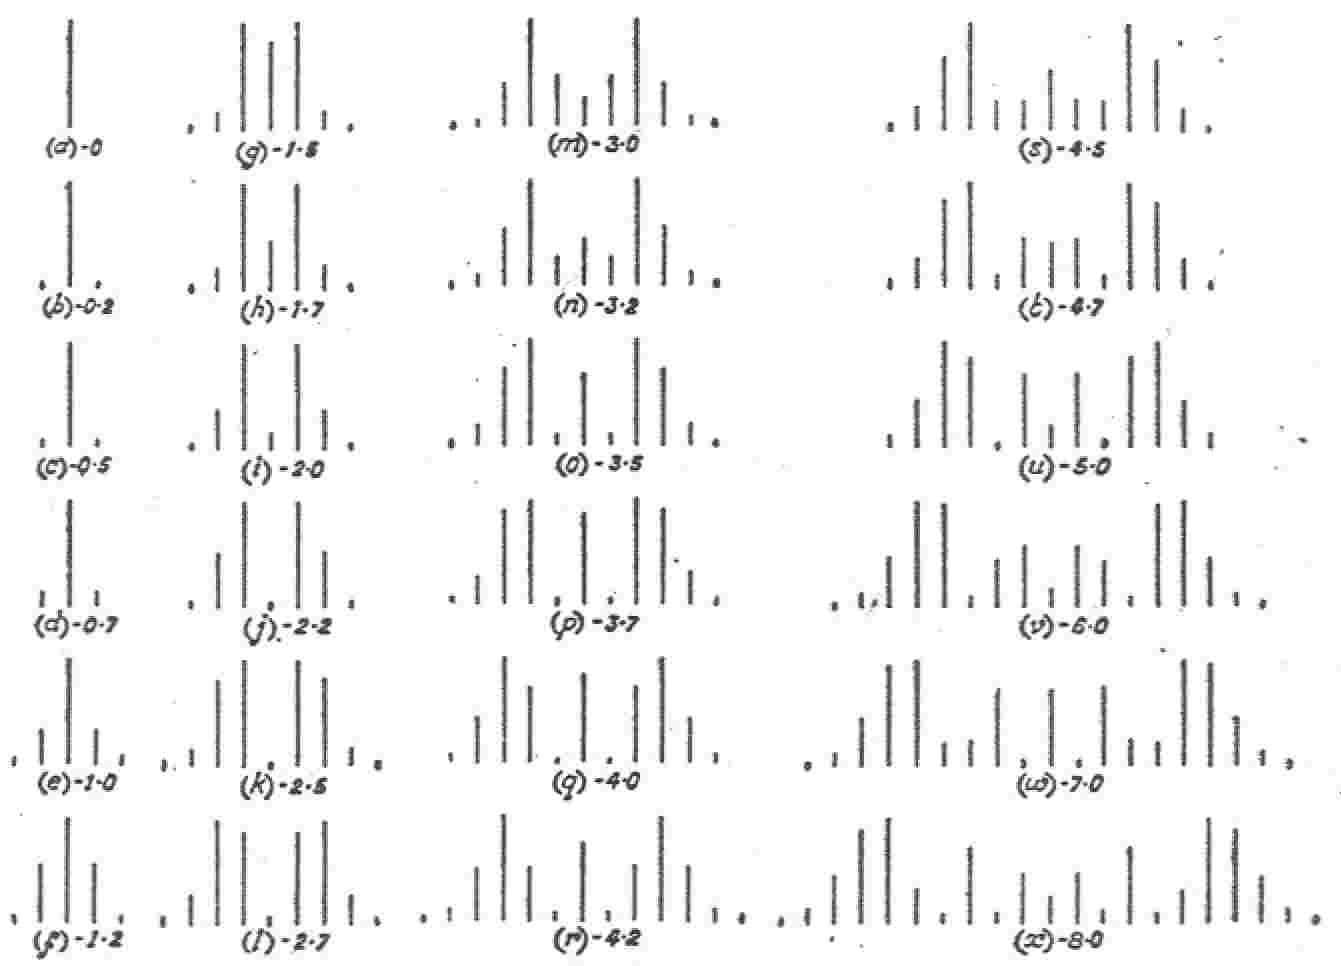
\includegraphics{Bilder/bessel-funktionen.jpg}
 \caption{Relative Intensitäten in Abhängigkeit von $v$ nach \cite{Raman}}
\end{figure}

